\section{Freifunk: die Idee}
\subsection{Über Freifunk}

\begin{frame}
\frametitle{Was ist Freifunk überhaupt?}
	\begin{itemize}
		\item \href{https://vimeo.com/64814620}{Video: Freifunk verbindet!}
		\item Aufbau eines vermaschten Netzwerkes $\rightarrow$ Meshnetz
		\item Demokratisierung einer Infrastruktur
		\item Zur Verfügung stellen freier Kommunikation für alle Personen $\leftrightarrow$ Offenes WLAN
		\item Netzneutralität
		\item Unabhängige \textbf{unkommerzielle Infrastruktur} in Bürgerhand
		\item Kostenlose, benutzerfreundliche \textbf{Hotspot-Gemeinschaft}
	\end{itemize}
\end{frame}

\begin{frame}
\frametitle{Wer macht Freifunk?}
	\begin{itemize}
		\item \textbf{Hierachiefreie}, \textbf{offene}, überregionale Gemeinschaft, die diese Grundsätze verfolgen will
		\item Personen, die \textbf{Router} aufstellen, \textbf{Firmware} schreiben oder \textbf{Server} bereitstellen
		\item Beginnt schon damit, dass eine Person einen Router für andere Menschen zur Verfügung stellt
		\item Unabhängige \textbf{unkommerzielle Infrastruktur} in Bürgerhand
		\item Dezentral weitflächig über Deutschland verteilt
	\end{itemize}
\end{frame}

\begin{frame}
\frametitle{Warum?}
	\begin{itemize}
		\item Flächendeckende innerstädtische \textbf{Internetversorgung}
		\item Teilen eines Internetzugangs \textbf{mit Nachbarn} (z.B. als Backup)
		\item Anbinden von \textbf{unterversorgten Gebieten} und Dörfern
		\item \textbf{Anonymes Netz} (Privatsphäre, Datenschutz, VDS)
		\item \textbf{Experimentelles }IPv4/IPv6 \textbf{Netzwerk }mit festen IPs
		\item \textbf{Lokale Dienste:} 
		\\ IP-Telefonie, OwnCloud, Wikis, Blogs, TV-Streaming, Kirchenfunk, Community-Radio, Chat, Online-Spiele, Lokale Nachrichten, usw..
	\end{itemize}
\end{frame}


\subsection{Wie funktioniert Freifunk?}

\begin{frame}
\frametitle{Wie funktioniert Freifunk?}
	\begin{itemize}
		\item WLAN-Mesh-Technologie “\textbf{Funk-Maschennetz}”
		\item Diese Technik eignet sich besonders gut um geografische und soziale Lücken zu schließen.
	\end{itemize}
	\begin{columns}[c]   
		\begin{column}[T]{0.4\textwidth}     
			\begin{itemize}
				\item \textbf{VPN vernetzt} „Inseln” und Städte
				\item Billig, Robust und ausfallsicher
				\item Für Alle immer frei und \textbf{unzensiert}
			\end{itemize}
		\end{column} 
		\begin{column}[T]{0.5\textwidth}     
			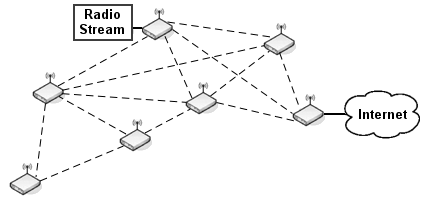
\includegraphics[width=\textwidth]{images/mesh_uebersicht.png}   
		\end{column}
	\end{columns} 
\end{frame}


\begin{frame}
\frametitle{Wohin geht welcher Traffic?}
	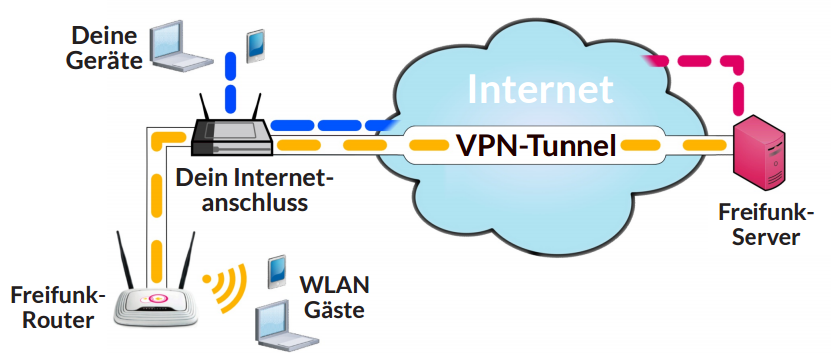
\includegraphics[scale=0.4]{images/personal_setup.png}
\end{frame}

\subsection{Das braucht man}
\begin{frame}
\frametitle{Das braucht man}
\begin{itemize}
\item Einen günstigen, unterstützen Router (ab ca. 17\euro)
\item Eine spezielle Firmware
\item Die Zustimmung zum \glqq Pico-Peering Agreement\grqq \footnotemark[1]
\begin{itemize}
\item Freier Transit
\item Offene Kommunikation
\item Keine Garantie (Haftungsausschluss)
\item Nutzungsbestimmungen
\item Lokale (individuelle) Zusätze
\end{itemize}
\end{itemize}
\footnotetext[1]{Regelwerk, über grundsätzlich Eigenschaften des Freifunks}
\end{frame}

\subsection{Juristisches}

\begin{frame}
\frametitle{Störerhaftung}
	\begin{itemize}
		\item WLan-Anbieter sind seit 2016 Haftungspriviligiert, Rechteinhaber können aber weiterhin auf Unterlassen klagen
		\item Keine Probleme durch Störerhaftung, da VPN Tunnel zum Freifunk Netzwerk
	\end{itemize}
\end{frame}
